\subsection{Features}
\label{sec:methods_features}


In this section, all the features of the model are introduced. We will present
univariate and bivariate analysis of the features as well as different
techniques to transform them, in particular fractional differentiation.

When working with inference models, features should be stationary. Common
procedures to features like prices involve integer differentiation to end up
working with price returns instead. The latter would remove entirely the price
series memory which is required by the model to effectively predict the output.
Other methods involve applying power transformations such as logarithms, square
roots or box-cox transformations. We are not interested in those for price series.
They will drastically affect scales and might collapse movements around the trend
while preserving the trend.

In \cite{frac_diff_paper} the fractional differentiation method was introduced,
and Lopez de Prado takes the method and explains the model in chapter 5 of
\cite{lopez_de_prado}. I will present the mathematical model and explain the
algorithm in what follows.

Let $B$ be a backshift operator, i.e. delay operator, to be applied to a matrix 
of real valued features $X_{t}$ such that $B^k X_t = X_{t-k}$. Also, we can 
express the positive integer powers of a binomial as $(x+y)^n = \sum_{k=0}^n {n \choose k} x^k y^{n-k}$.
When considering real valued exponents, combinatorial number ${n \choose k}$
becomes (after substitution of $n$ an integer by $d$ a real number) ${d \choose k} = \frac{d (d-1) ... (d-k+1)}{k!}$
which coincides with the integer formula. Thus,

\begin{equation}
  \label{eqn:binomial_expantion_frac_power}
  (x+y)^d = \sum_{k=0}^{\infty} {d \choose k} x^k y^{d-k}
\end{equation}

Equation \ref{eqn:binomial_expantion_frac_power} presents an infinite series, a
key difference with respect to the integer counterpart. If we replace $x$ by $1$
and $y$ by $-B$, the backshift operator, one can write from \ref{eqn:binomial_expantion_frac_power}:

\[(1-B)^d = \sum_{k=0}^{\infty} {d \choose k} (-B)^k \]

\[(1-B)^d = \sum_{k=0}^{\infty} \frac{\prod_{i=0}^{k-1}(d-i)}{k!} (-B)^k \]

\begin{equation}
  \label{eqn:binomial_expantion_diff_operator}
  (1-B)^d = 1 - dB + \frac{d(d-1)}{2!}B^2 - \frac{d(d-1)(d-2)}{3!}B^3 + ...
\end{equation}

Equation \ref{eqn:binomial_expantion_diff_operator} presents the foundation of
the fractional differentiation method. If one could find the value of $d$ such
that a series $X$ gets differentiated and becomes stationary while preserving
as much memory as possible a later model would be able to exploit that memory to
predict the output. In particular, when the value of $d$ ends up being less than 1.
Equation \ref{eqn:binomial_expantion_diff_operator} also
presents a problem, it is a infinite series when $d$ is noninteger which makes
the operation to be non exact for the general case due to the impossibility of
applying infinite multiplications and sums. Lopez de Prado proposes a solution
for both issues.

A fractionally differentiated series $X$ can be expressed for a given $d$ as: 

\[ X_t^d = \sum_{k=0}^{\infty} w_k X_{t-k} \]

The vector $w$ of weights in the above equation follows:

\begin{equation}
  \label{eqn:ffd_weights}
	w = {1, -d, \frac{d(d-1)}{2!}, -\frac{d(d-1)(d-2)}{3!}, ..., (-1)^k \prod_{i=0}^{k-1} \frac{(d-i)}{k!}} 
\end{equation}

One can derive by inspection of equation \ref{eqn:ffd_weights} a generative and
recursive expression for each item in the series:

\begin{equation}
  \label{eqn:ffd_weights_generative}
  w_k = -w_{k-1} \frac{d-k+1}{k}
\end{equation}

Equation \ref{eqn:ffd_weights_generative} is easy to implement as a programming
function which is ideal for this application. It is also interesting to evaluate
the tendency of $w_k$ as $k$ tends to infinite, see figure \ref{fig:w_k_vs_k}.

\begin{figure}[!htb]
    \centering
    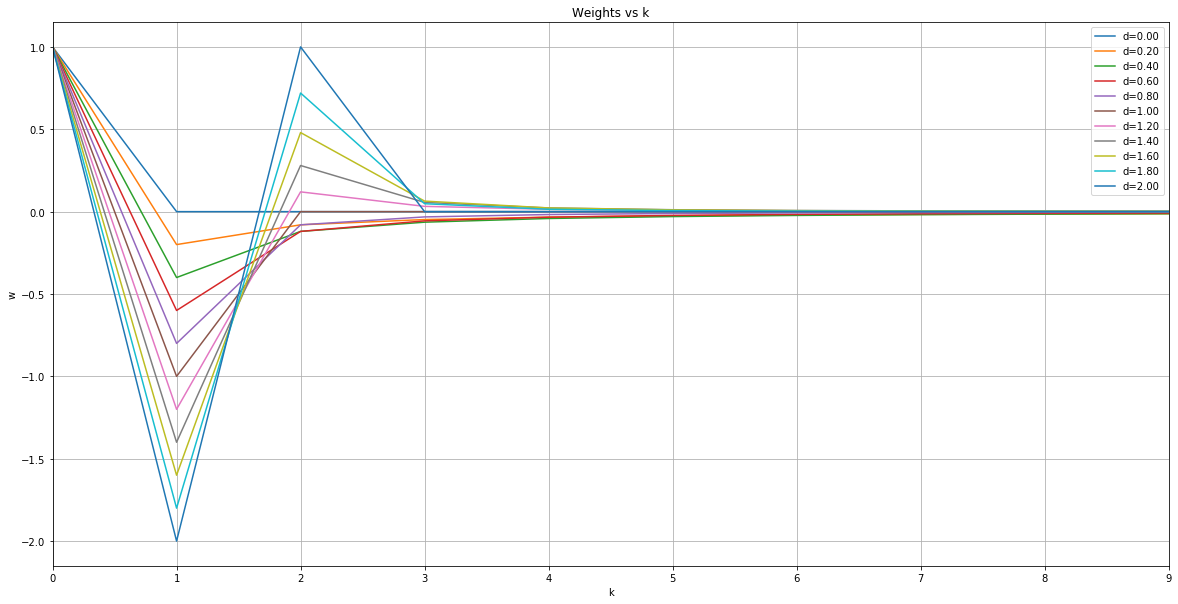
\includegraphics[width=\textwidth]{methods/images/weights_vs_k.png}
    \caption{Weight values vs. $k$ for different $d$ values.}
    \label{fig:w_k_vs_k}
\end{figure}

As it can be seen in figure \ref{fig:w_k_vs_k}, coefficients tend to zero as $k$
increases. It can also be proved the convergence of coefficients $w_k$. Let's
analyze the following when $k > d$ and $w_{k-1} \ne 0$:

\[|\frac{w_k}{w_{k-1}}| = |\frac{d-k+1}{k}| < 1 \]

what makes $|w_k| < |w_{k-1}|$ leading to $\lim_{k \to \infty} w_k = 0$.

When implementing fractional differentiation on a real time series, one has two
options:

\begin{enumerate}
  \item Adjust the length of $w_k$ vector by weight loss with a certain
        threshold.
  \item Work with a fixed number of coefficients.
\end{enumerate}

Option 1 requires the operation to compute the size of $w_k$ vector to account
for weight loss given a certain threshold. Weight loss cam be computed:

\begin{equation}
  \lambda_l = \frac{\sum_{j=T-l}^{T}|w_j|}{\sum_{i=0}^{T-1}|w_i|}
\end{equation}

where:

\begin{itemize}
  \item $T$ is the length of the time series,
  \item $l$ is the index of the sample from the end where the fractional
        differentiation occurs.
  \item $\lambda_l$ the weight loss at $l$ index
\end{itemize}

One should discard all samples whose $\lambda_l < \tau$ and $\tau$ is the
threshold. As $d \to 0$, the energy of the weights decreases leading to more
weight loss and more discarded samples.

Option 2 comes with the simplicity of having always the same vector of
coefficients $w_k$ such that $|w_k| > \tau$ and $\tau$ is a user defined
threshold. It comes with the advantage of having no drift as option 1 and just
needs to drop $l$ samples at the beginning, being $l$ the value of $l$ that
makes $w_k$ less or equal to $\tau$. In this thesis, option 2 is used.

So far, how to compute the weights vector was explained. Now, we just need to
address the value of $d$. $X_t$ might be stationary already which leads to
$d^* = 0$ with $d^*$ the value of $d$ that preserves most memory making the 
time series stationary. When $X_t$ has a \emph{unit root} (see chapter 15 of \cite{time_series_analysis}),
$0 \le d^* \leq 1$. And when $X_t$ exhibits an explosive (bubble) behavior,
$d^* > 1$. Unit roots can be tested with Dickey Fuller hypothesis test
(see chapter 17 of \cite{time_series_analysis}). The null hypothesis of the test claims the series has a unit root.
After determining a certain confidence level one can derive an \emph{optimum}
$d^*$ by:

\begin{enumerate}
  \item Define a vector of $d$ values in range of 0 to 1.
  \item For each value of $d$:
  \begin{enumerate}
    \item Fractionally differentiate $X_t$ with $d$ given a certain amount of
          weights. Obtain $X_t^d$.
    \item Compute the Dickey Fuller statistic, ADF, for $X_t^d$.
    \item Compute the p-value of the test.
  \end{enumerate}
  \item Choose $d^*$ that yields the maximum p-value between all p-values that
        are less or equal to the confidence level.
\end{enumerate}

This process has two flaws:

\begin{itemize}
  \item It is computationally time complex. Each time we apply the fractional
        differentiation, we are processing a $O(n^2)$ algorithm. Computing the
        ADF of the differentiated series requires a differentiation and model
        estimation which yields at least another $O(n^2)$ process. Finally, we
        iterate through a vector of $d$ adding another dimension.
  \item \emph{Optimum} $d$ is subject to the granularity of the $d$ vector of
        samples. The smaller the step, the more information one could preserve
        in the final time series, but the more iterations are required which
        impacts directly in the aforementioned item.
\end{itemize}

Regardless, all features that expose non-stationary characteristics could be
transformed and stabilized while preserving memory.